\newpage
\section{RC-circuit}
Consider the following electrical circuit:
\begin{center}
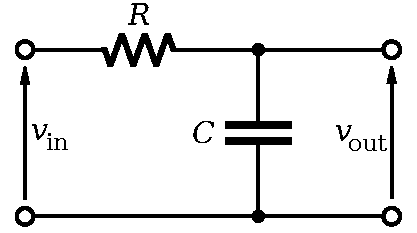
\includegraphics[width=0.5\textwidth]{Applications/figures/rc.pdf}
\end{center}
This is a very simple analogue filter implemented using a resistor and
a capacitor. This type of a circuit is used often in e.g., audio
electronics to remove high pitched signals.

This system can be modeled as a linear time-invariant system. In this
case $v_{\mathrm{in}}(t) = x(t)$ and $v_{\mathrm{out}}(t) =
y(t)$. This system has the following impulse response:
\begin{equation}
h(t) = \frac{1}{RC} e^{-\frac{1}{RC}t}u(t) = \alpha e^{-\alpha t} u(t)
\end{equation}
where the real valued constant $\alpha > 0$. 

In order to determine the frequency response, we evaluate the Fourier 
transform of the impulse response:
\begin{align}
\Hiw &= \int_{-\infty}^{\infty} \alpha e^{-\alpha t} u(t) e^{-i\omega t}dt \\
     &= \alpha \int_{0}^{\infty} e^{-(\alpha+i\omega) t} dt \\
     &= \alpha \left. \frac{e^{-(\alpha+i\omega)t}}{-(\alpha+i\omega)}\right\rvert_{t=0}^{\infty} \\
     &= \frac{\alpha}{\alpha + i\omega}\,\,.
\end{align}
In order to find the magnitude response, we'll need to establish that
\begin{equation}
  \mathcal{H}^*(\omega) = \frac{\alpha}{\alpha - i\omega}\,\,,
\end{equation}
which is relatively easy to show\footnote{For example using: \begin{equation*}\frac{\alpha}{\alpha + i \omega} = \frac{\alpha(\alpha - i\omega)}{\alpha^2 + \omega^2} = \frac{\alpha^2}{\alpha^2 + \omega^2} - i\frac{\alpha\omega}{\alpha^2 + \omega^2}\end{equation*}}.

The magnitude response is then:
\begin{align}
|\Hiw| &= \sqrt{\Hiw\mathcal{H}^*(\omega)}\\
       &= \frac{\alpha}{\sqrt{\alpha^2 + \omega^2}}\,\,.
\end{align}
The phase response is\footnote{recall that $\tan^{-1}(-x) = -\tan^{-1}(x)$}:
\begin{align}
\angle \Hiw &= \tan^{-1}{\frac{\mathrm{Im}(\Hiw)}{\mathrm{Re}(\Hiw)}} \\
            &= - \tan^{-1}{\frac{\omega}{\alpha}}\,\,.
\end{align}
The magnitude and phase responses are plotted below:
\begin{center}
\begin{minipage}{.49\textwidth}
\begin{tikzpicture}
	\begin{axis}[domain=(-150):(150),samples=200,ymax=1.2,
        xlabel={$\omega$},
        ylabel={$|\Hiw|$},
        axis x line=center, 
        axis y line=middle,
        ytick={0.707,1.0},
        yticklabels={$\frac{1}{\sqrt{2}}$,$1$},
        xtick={-40,40},
        xticklabels={$-\alpha$,$\alpha$}
    ]
        \addplot [dashed,black] coordinates { (-40,0.0) (-40,0.707) };
        \addplot [dashed,black] coordinates { (40,0.0) (40,0.707) };
        \addplot [dashed,black] coordinates { (-40,0.707) (40,0.707) };
        
	\addplot[blue] {40/sqrt(x*x+40*40)};
    \end{axis}
\end{tikzpicture}
\end{minipage}
\begin{minipage}{.49\textwidth}
\begin{tikzpicture}
	\begin{axis}[domain=(-150):(150),samples=200,ymin=-100,ymax=100,
        xlabel={$\omega$},
        ylabel={$\angle \Hiw$},
        axis x line=center, 
        axis y line=middle, 
        ytick={-90,-45,45,90},
        yticklabels={$-\frac{\pi}{2}$,$-\frac{\pi}{4}$,$\frac{\pi}{4}$,$\frac{\pi}{2}$},    
        xtick={-40,40},
        xticklabels={$-\alpha$,$\alpha$}    
    ]
    \addplot[blue] {-atan(x/40.0)};
    \addplot[dashed,blue] {-180*x/40.0/3.14};
\addplot [dashed,black] coordinates { (-40,0.0) (-40,45) };
        \addplot [dashed,black] coordinates { (40,0.0) (40,-45) };
        \addplot [dashed,black] coordinates { (-40,45) (0,45) };
        \addplot [dashed,black] coordinates { (40,-45) (0,-45) };

\end{axis}
\end{tikzpicture}
\end{minipage}
\end{center}
Note that the ``half-power'' point, where $|\Hiw|^2=\frac{1}{2}$
corresponds to $\omega = \pm \alpha$. This half power width of a
filter is often referred to as the full width half maximum (FWHM). At
this ``half-power'' point, the phase is $- \tan^{-1}(\pm 1)
= \mp \frac{\pi}{4}$. For our example filter, the output power has
dropped to half when the frequency is:
\begin{equation}
\omega = 2\pi f = \frac{1}{RC}
\end{equation}
or 
\begin{equation}
f = \frac{1}{2\pi RC}\,\,.
\end{equation}
For example, if $R=1$ k$\Omega$ and $C=100$ pF, the cutoff frequency
of the filter is 1.6 MHz.

When looking at the Taylor series expansion of the phase around zero,
recalling that
\begin{equation}
\frac{d}{d\omega}\tan^{-1}(-\omega/\alpha) = \frac{\alpha}{\omega^2 + \alpha^2}\,\,,
\end{equation}
we get
\begin{equation}
\angle\Hiw \approx -\frac{1}{\alpha}\omega = -RC \omega\,\,.
\end{equation}
This is shown as a dashed blue line in the figure above. 

If we compare this with the equation for delay of a sinusoid
$x(t)=Ae^{i\omega t}$, which we can derive from
\begin{equation}
x(t-t_0) = Ae^{i\omega(t-t_0)} = Ae^{i\omega t} e^{-i\omega t_0} = Ae^{i\omega t} e^{i\varphi} 
\end{equation}
to be $-\omega t_0 = -RC\omega$, we see that the filter corresponds to
approximately a $t_0 = RC$ second time delay. This approximation is
valid for low values of $|\omega| < \frac{1}{2}\alpha$. In the case of
$R=1$ k$\Omega$ and $C=100$ pF, the time delay is approximately: 0.1
$\mu$s.



